\section{Introduction}
\label{intro}
% Many social, biological, and information systems can be naturally represented as networks -
% the elementary units of the system are reduced to nodes,
% while their relations and interactions are pictured as edges (or called links).

Communities are defined as groups of nodes that are more densely connected to each other than to the rest
of the network. The goal of the community detection algorithms, consequently, is to partition the networks
into groups of nodes; large body of work exists on community detection in single and isolated
network~\cite{fortunato2010community}. Recently, many real networks, including communication, social,
infrastructural and biological
ones, are often represented as multilayer networks~\cite{buldyrev2010catastrophic}.
A multilayer network is comprised of multiple interdependent networks, where each network layer represents one
aspect of interaction. Moreover, the functionality of a node in one network layer is dependent on the role of nodes in other layers.
For instance, a location based social networks (say, Yelp) can be represented as a multilayer network (see Fig.~\ref{yelp}) where in
one layer customers (visitors) are connected via social links and in the other layer location nodes are connected through proximity links.
The (coupling) link connecting a customer with a location node represents the visit of a customer to a location.
\begin{figure}
\centering
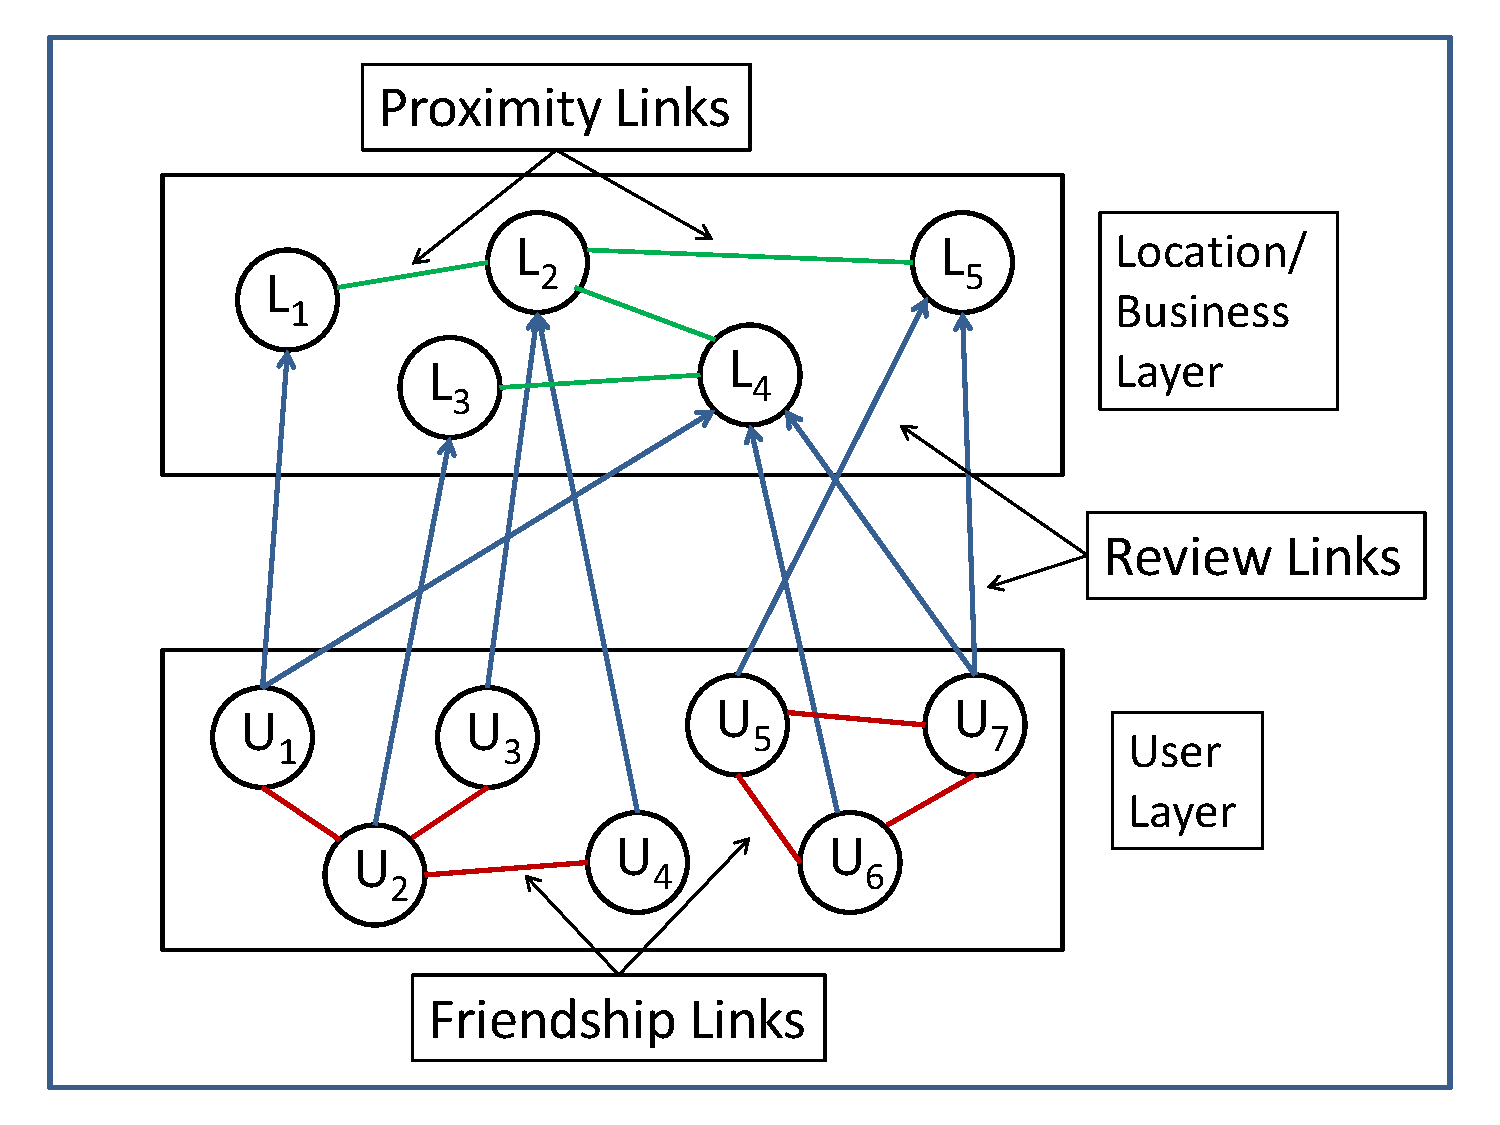
\includegraphics[width=2.3in]{./images/yelp_data.pdf}
\vspace{-0.1in}
\caption{A sample multilayer (Yelp) network.}
\vspace{-0.23in}
\label{yelp}
\end{figure}



% \begin{figure}
% \begin{center}
% \subfigure[A sample Yelp network
% ]{\label{nmi1}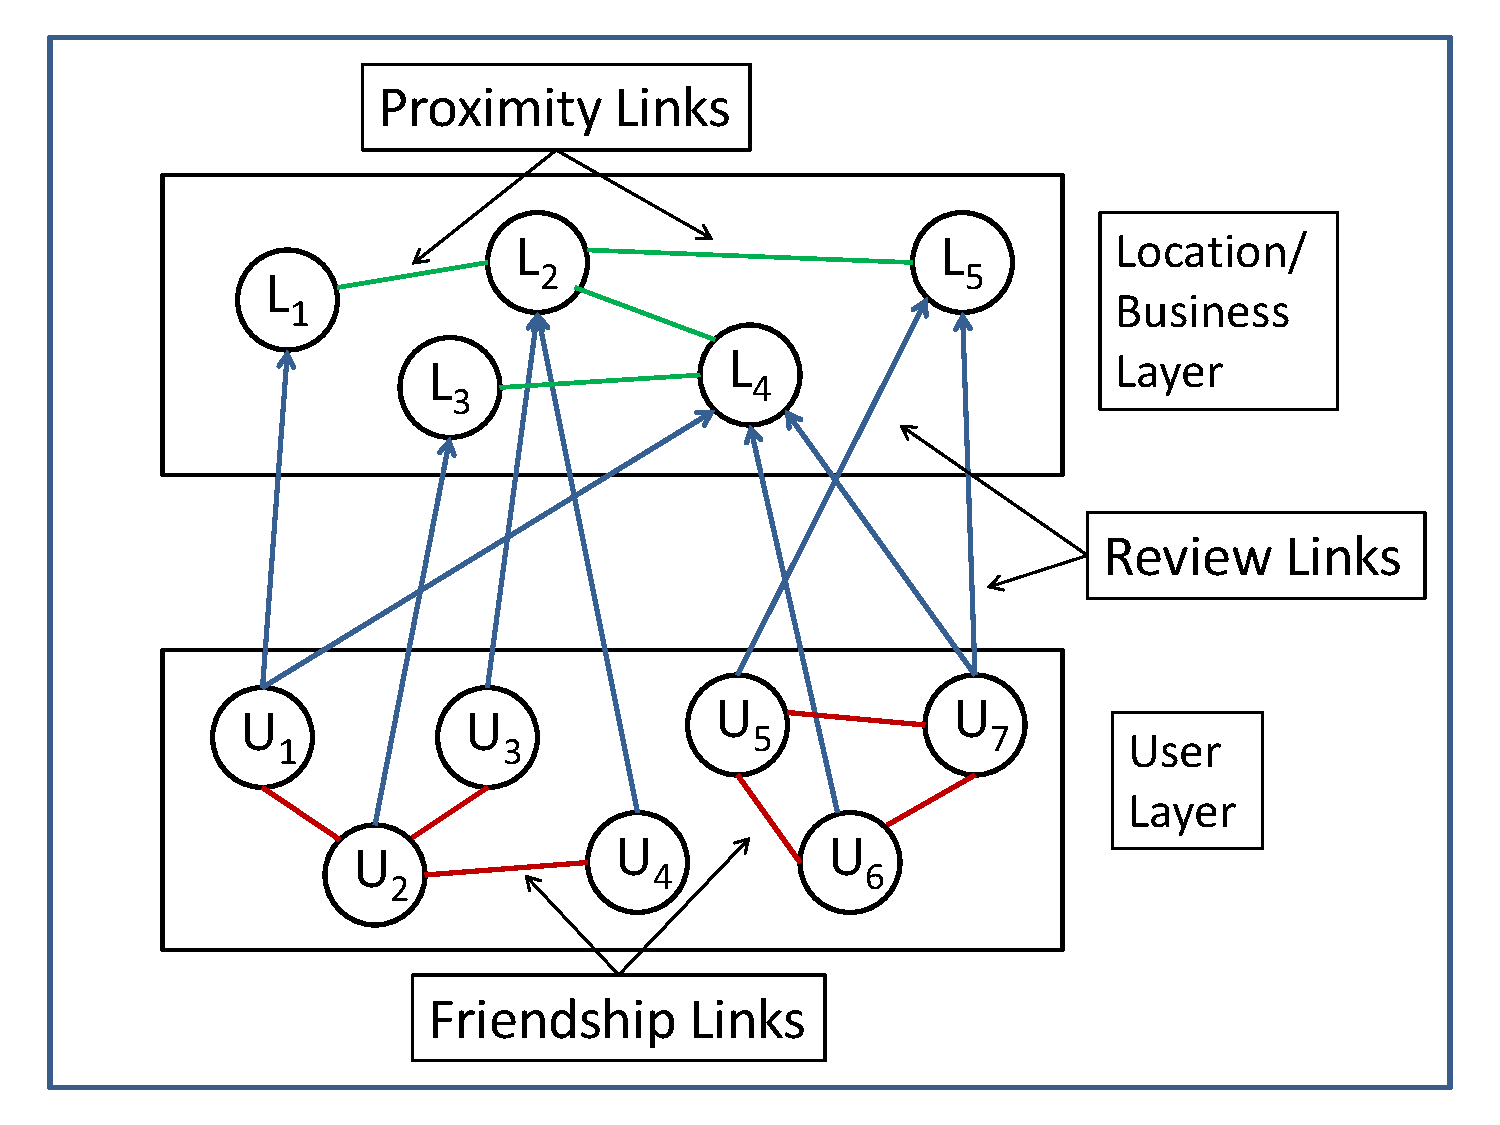
\includegraphics[angle=0,scale=.18]{./images/yelp_data.pdf}}
% \subfigure[A sample multilayer network with two different types of communities
% ]{\label{nmi1_1}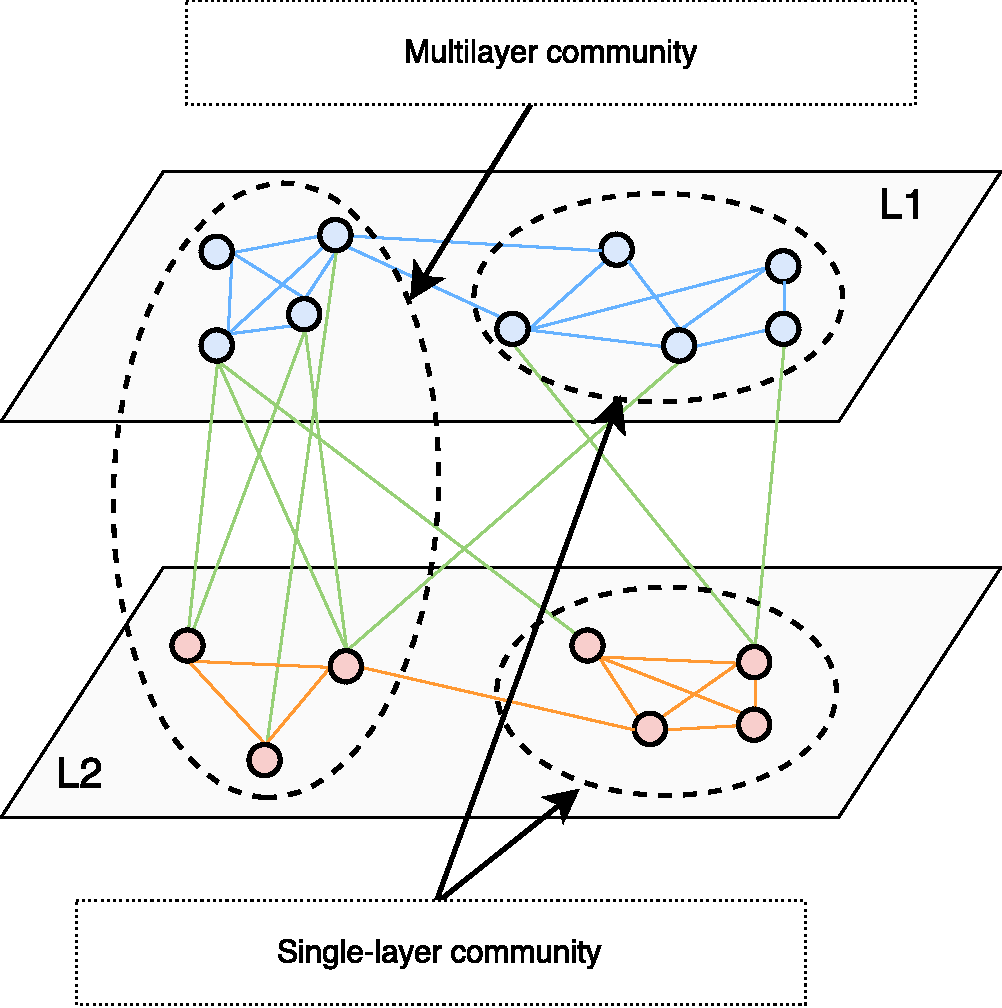
\includegraphics[angle=0,scale=.18]{./images/single_multi_community.pdf}}
% \end{center}
% \vspace{-0.1in}
% \caption{Sample multilayer networks}
% \vspace{-0.2in}
% \label{nmi00}
% \end{figure}



% \begin{figure*}
% \begin{center}
% \subfigure[A sample Yelp network
% ]{\label{yelp}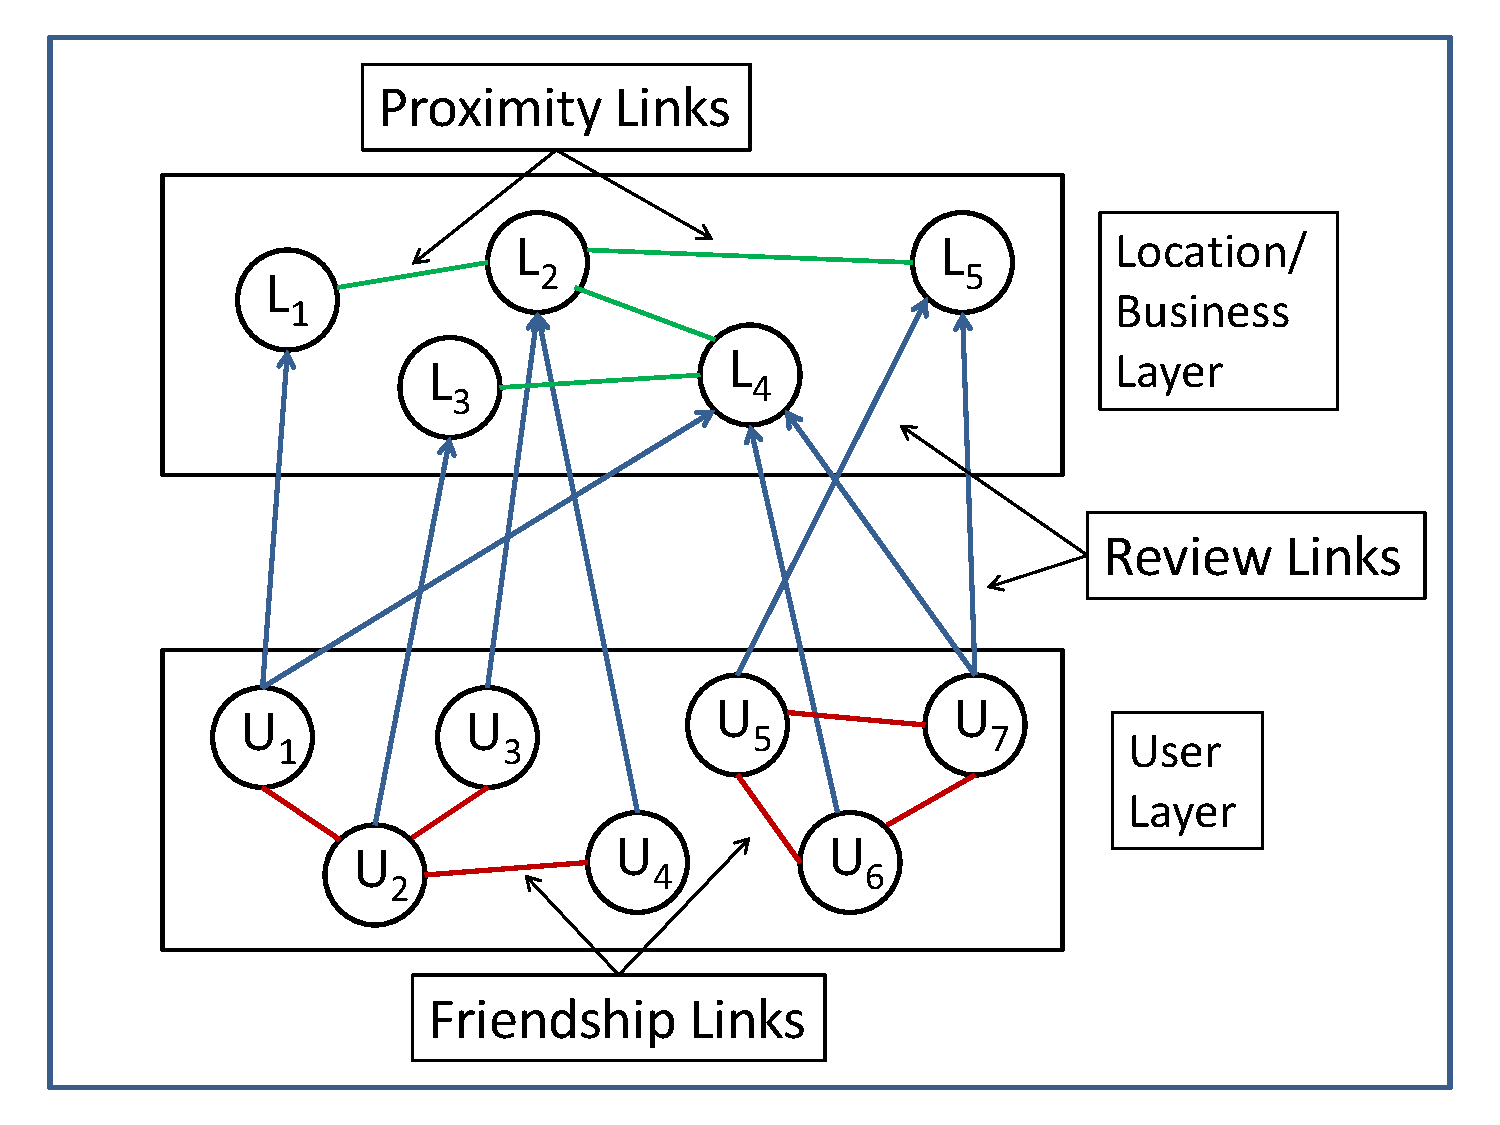
\includegraphics[angle=0,width=2.2in, height=1.5in]{./images/yelp_data.pdf}}
% \subfigure[Network configuration with two different ground truth communities
% ]{\label{N0}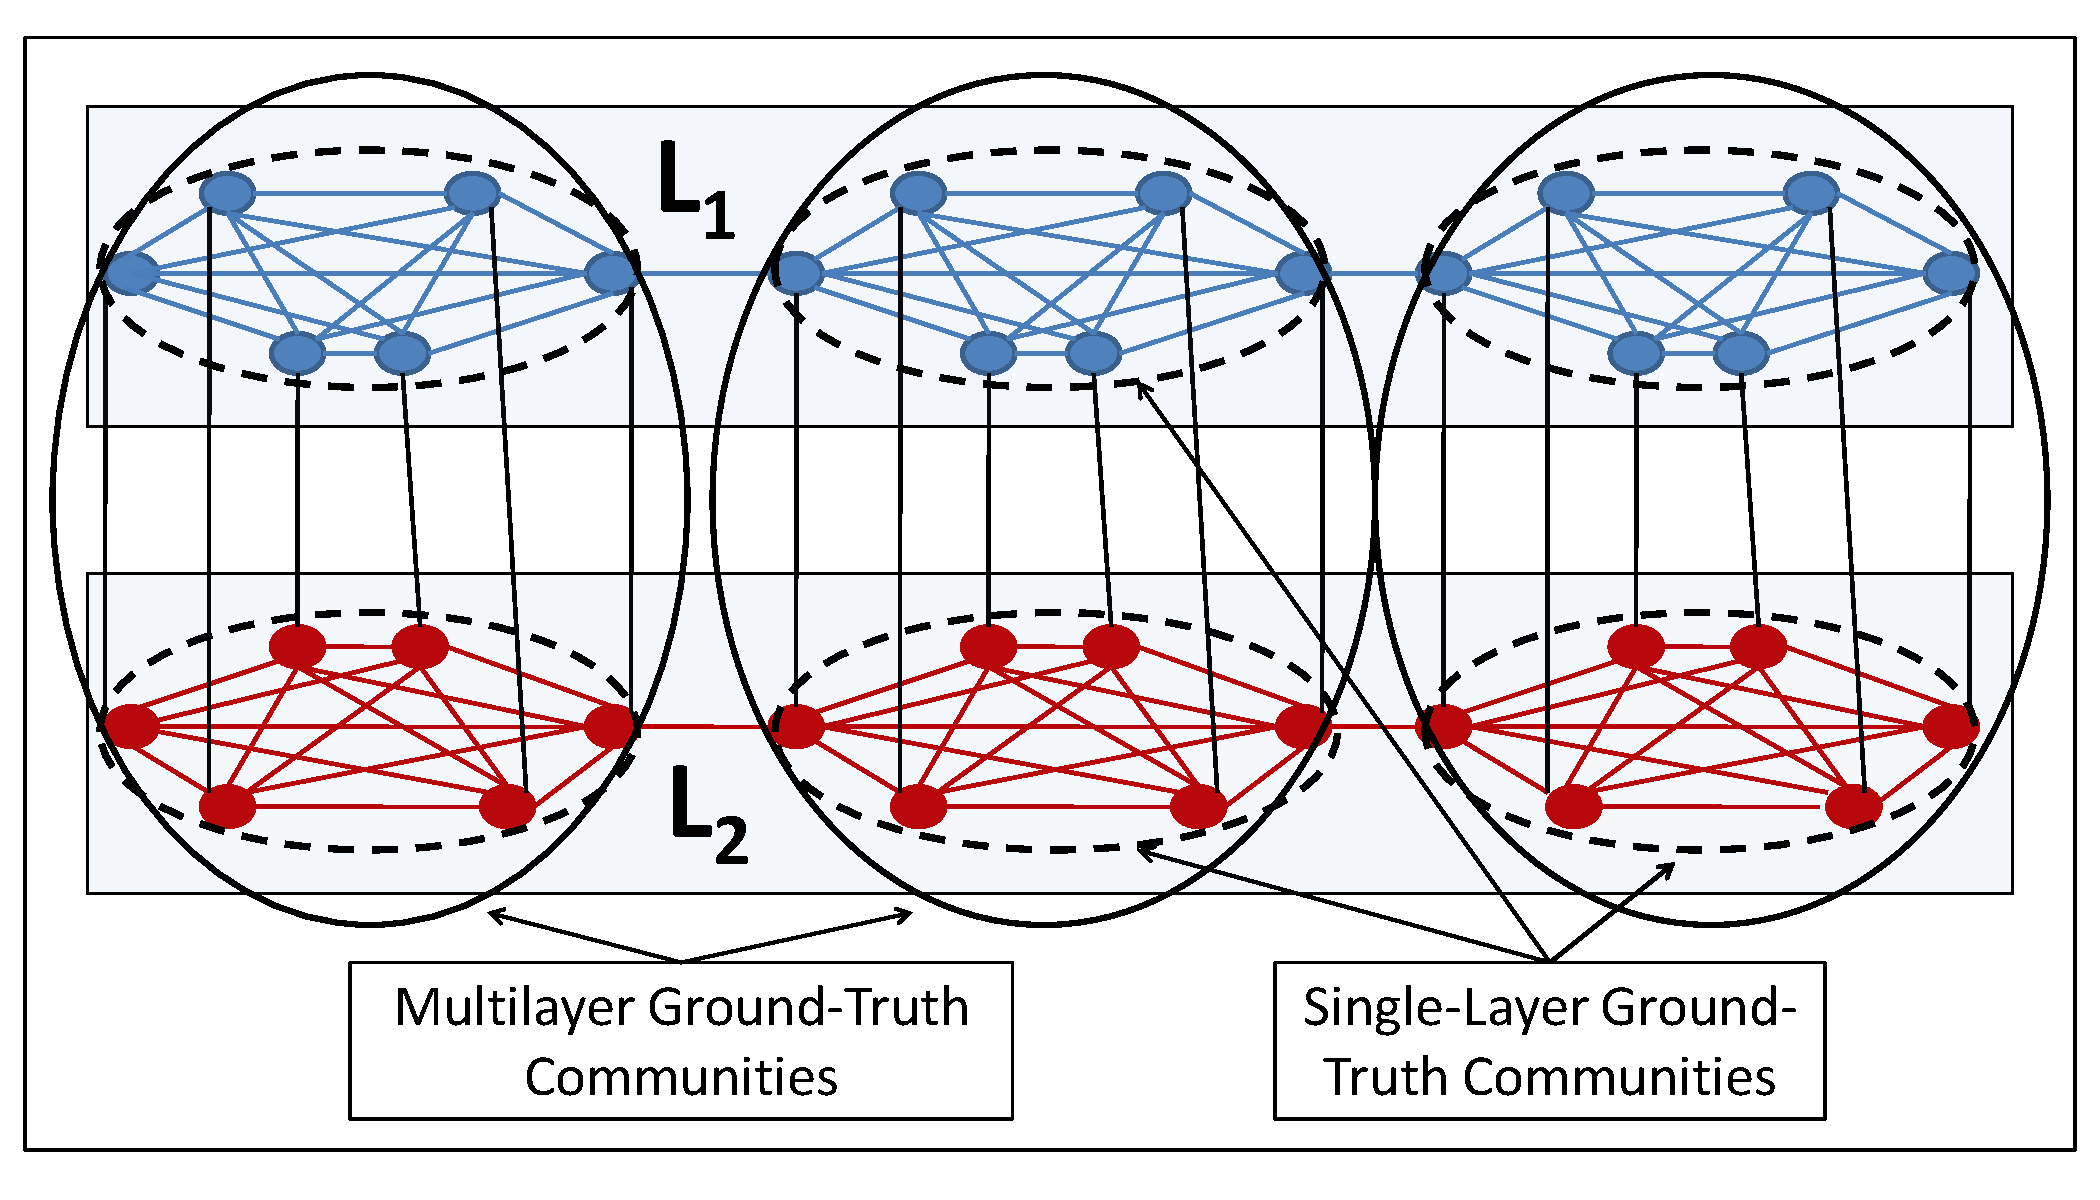
\includegraphics[angle=0,width=2.5in, height=1.5in]{./images/image31.pdf}}
% \end{center}
% \vspace{-0.25in}
% \caption{}
% \vspace{-0.2in}
% \label{YN0}
% \end{figure*}

% \begin{figure*}
% \centering
% 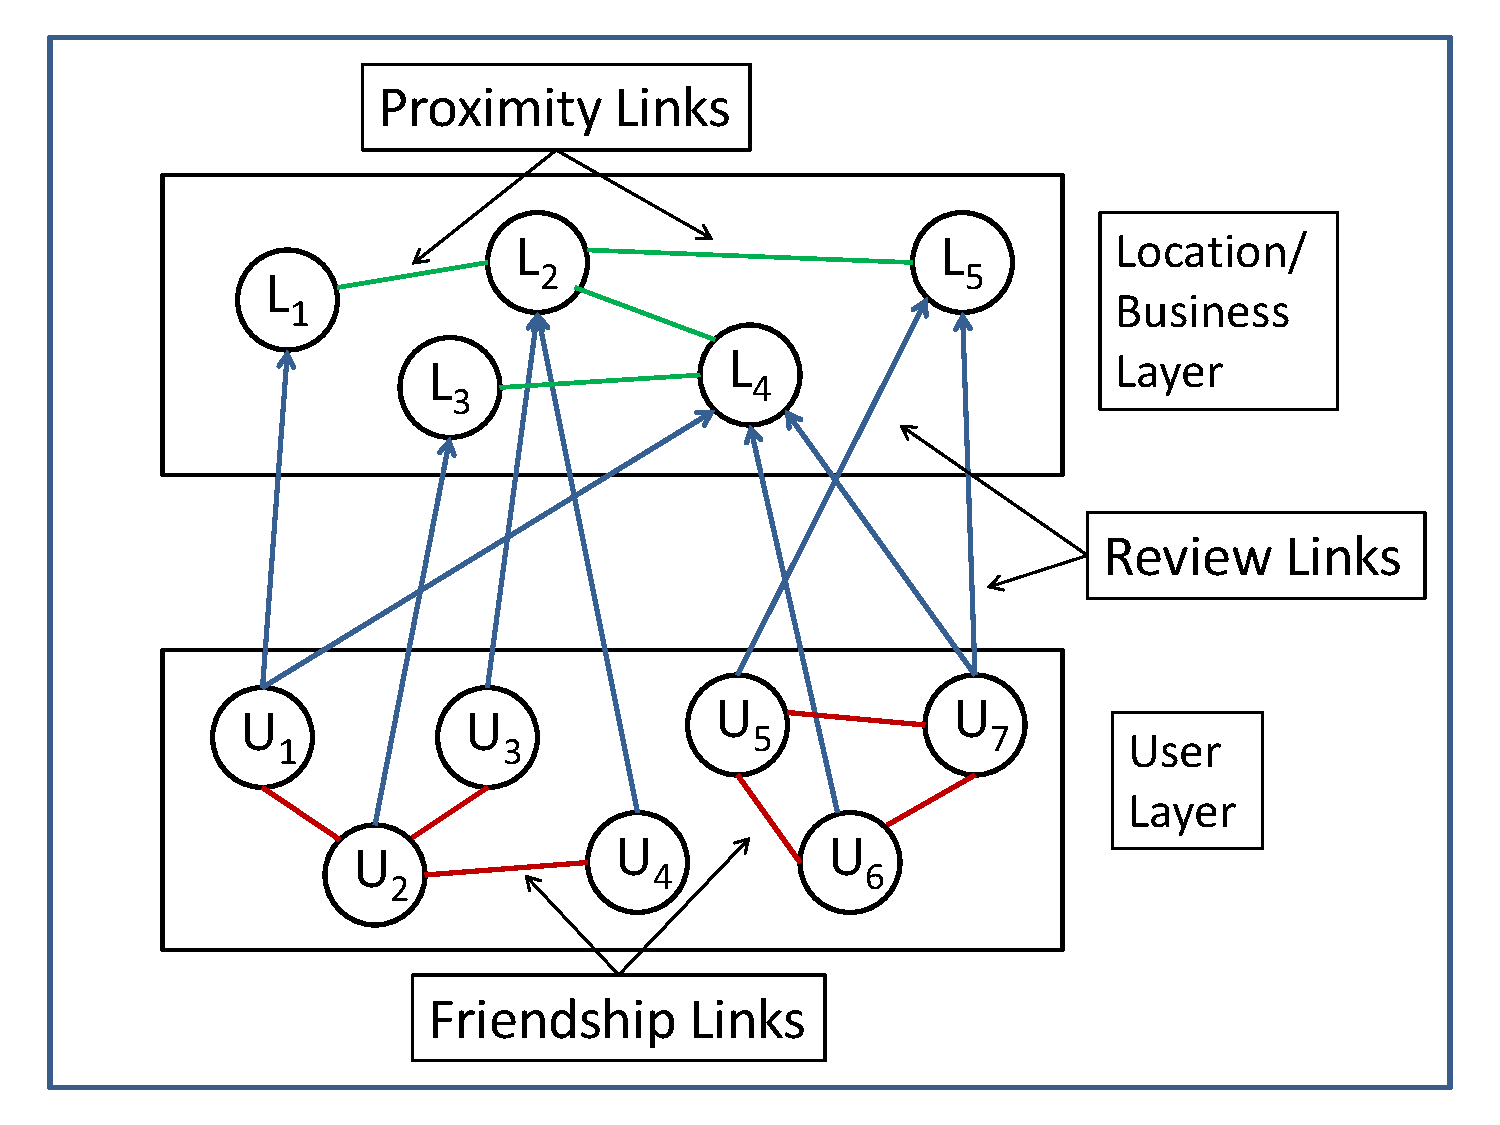
\includegraphics[width=2.5in]{./images/yelp_data.pdf}
% \vspace{-0.2in}
% \caption{A sample Yelp network}
% \vspace{-0.2in}
% \label{yelp}
% \end{figure*}

Community detection in complex multilayer networks is an important research problem.
%As we know, community detection i.e. the task of grouping objects based on their similarity, is one of the most important data mining tasks.
The communities in multilayer networks help to identify
functionally cohesive sub-units and reveal complex interactions between multi-type nodes
and heterogeneous links. They are also found to be beneficial for different
data mining tasks such as context-sensitive search, prediction and recommendation etc~\cite{metafac}. %[BM: need 1-2 good lines].
%provide an insight into how the system is internally organized~\cite{fortunato2010community,gulbahce2008art}. Such an analysis can also shed some light on the dynamics of group formation in the presence of heterogeneous interactions.
Community detection in multilayer network is challenging as the detected communities have possibility to contain only single or
multiple types of nodes.
Most of the recent endeavors concentrated on the
multiplex networks~\cite{mucha2010community,kuncheva2015community} where all layers share the
identical set of nodes but may have multiple types of interactions. In multiplex network, some of the approaches propose new quality
metrics~\cite{mucha2010community} to measure the goodness of the detected communities
%some approaches discover communities in each layer separately and then perform a frequent-pattern mining~\cite{berlingerio2013abacus}
whereas a few other
approaches utilize random walk~\cite{kuncheva2015community}
or frequent-pattern mining techniques~\cite{berlingerio2013abacus}
to obtain structurally similar components.
% There exists another school of
% research which discovers the communities in each layer separately and then perform a frequent-pattern mining~\cite{berlingerio2013abacus}.
In principle, most of the aforementioned algorithms transform the problem to the classical community detection in a monoplex network
leveraging on the fact that in multiplex network, one-to-one cross layer links connect the copies of the same nodes in multiple
layers. Unfortunately, the presence of heterogeneous nodes across multiple layers and cross layer dependency links make the
aforementioned solutions
inadequate for multilayer networks.
% Precisely, the communities detected in multiplex network possess only a single type of
% nodes which makes them difficult to extend for multilayer networks due to the presence of multiple types of nodes.

% collapse all the layers of the network into a single one and apply standard single layer community detection
% algorithms~\cite{rosvall2008maps,schuetz2008efficient,newman2004fast,duch2005community,clauset2004finding,newman2004finding,blondel2008fast} whereas.......
% [BM: need 1-2 lines summarizing the techniques of the multiplex comm detection]
%The naive approach is to collapse all the layers of the network into a single one and apply standard single layer community detection
%approaches~\cite{rosvall2008maps,schuetz2008efficient,newman2004fast,duch2005community,clauset2004finding,newman2004finding,blondel2008fast}.However, this approach suffer from massive information loss. [BM: one more line on the multiplex comm detection]



 %[BM: replace ineffective by a better word]

Attempts have been made in bits and pieces to detect communities in multilayer networks; novel methodologies have been
introduced such as Dirichlet % and non-negative matrix factorization~\cite{comar2012framework},
process~\cite{sun2014co}, tensor factorization~\cite{metafac}, subspace clustering~\cite{dong2014clustering},
non-negative matrix factorization~\cite{Cheng_kdd13} etc.
%and block model analysis~\cite{tang2012identifying} [BM: so many work? Want to reduce?].
% [BM: previous line is not clear.
% Need one good line to highlight the limitation. I write the following, but you try to add/revise.]
% However, most of these approaches suffer from several limitations.
% Some only work on a specific type of multilayer networks (say, star-type etc.)
% or are unable to detect communities comprising of multiple and single types of nodes simultaneously,
% others require to fix the number of communities apriori, limiting their capability to discover of the true set of communities.
% Finally, a proper framework to generate benchmark communities for generic multilayer network is not available for any of them.
However, most of these approaches suffer from several limitations. First of all, some of the aforesaid algorithms only work
on a specific type of multilayer networks (say, star-type~\cite{sun2014co} etc.). Secondly, some of them are
forced to detect communities comprising only multiple types of nodes~\cite{metafac}, hence introducing bias. Third, the desired number of
communities are required to be fixed apriori for most of them~\cite{metafac,dong2014clustering},
limiting their capability to discover the true set of communities.
Finally, a proper framework to generate benchmark communities for generic multilayer network is not available in any of them.

%
% Third, the desired number of communities are required to be fixed apriori for most of them,
% limiting their capability to discover of the true set of communities.
% Finally, a proper framework to generate benchmark communities for generic multilayer network is not available in any of them.

% Few attempts have been made in proposing modularity index for multilayer networks.
% Composite modularity~\cite{CompMod} calculates
% the modularity of a multi-relational network as the integration of modularities calculated for each single-relational subnetwork.
% However, due to the deficiency in definition,
% the composite modularity can only produce communities with single type of nodes. On the other side, modularity
% proposed in~\cite{medical_paper} in the context of gene-chemical interaction network fails to conceive the role of coupling links
% in community characterization.
% The detailed exploration of prior art reveals the importance of the multilayer community
% detection algorithm which is free from (a). any external parameter, say total number of communities (b). any bias towards
% communities with only single type or only multiple types of nodes.
% % The exploration of prior art reveals the importance to develop a proper modularity index that should tackle the limitations
% % discussed above.
% Developing a proper modularity index should be the first
% step towards this direction.

Recent endeavors directed towards development of modularity index for heterogeneous networks.
For instance, composite modularity~\cite{CompMod} calculates
the modularity of a multi-relational network as the integration of modularities calculated for each single-relational subnetwork.
However, due to the deficiency in definition,
the composite modularity can only produce communities with single type of nodes. On the other side, modularity
proposed in~\cite{medical_paper} in the context of gene-chemical interaction network fails to conceive the role of coupling links
in communities characterization. The detailed exploration of prior art reveals the importance of the multilayer community
detection algorithm which is free from (a) any external parameter, say total number of communities (b) any bias towards
communities with only single type or only multiple types of nodes. Developing a suitable modularity index should be the first
step towards this direction.

\begin{figure}
\centering
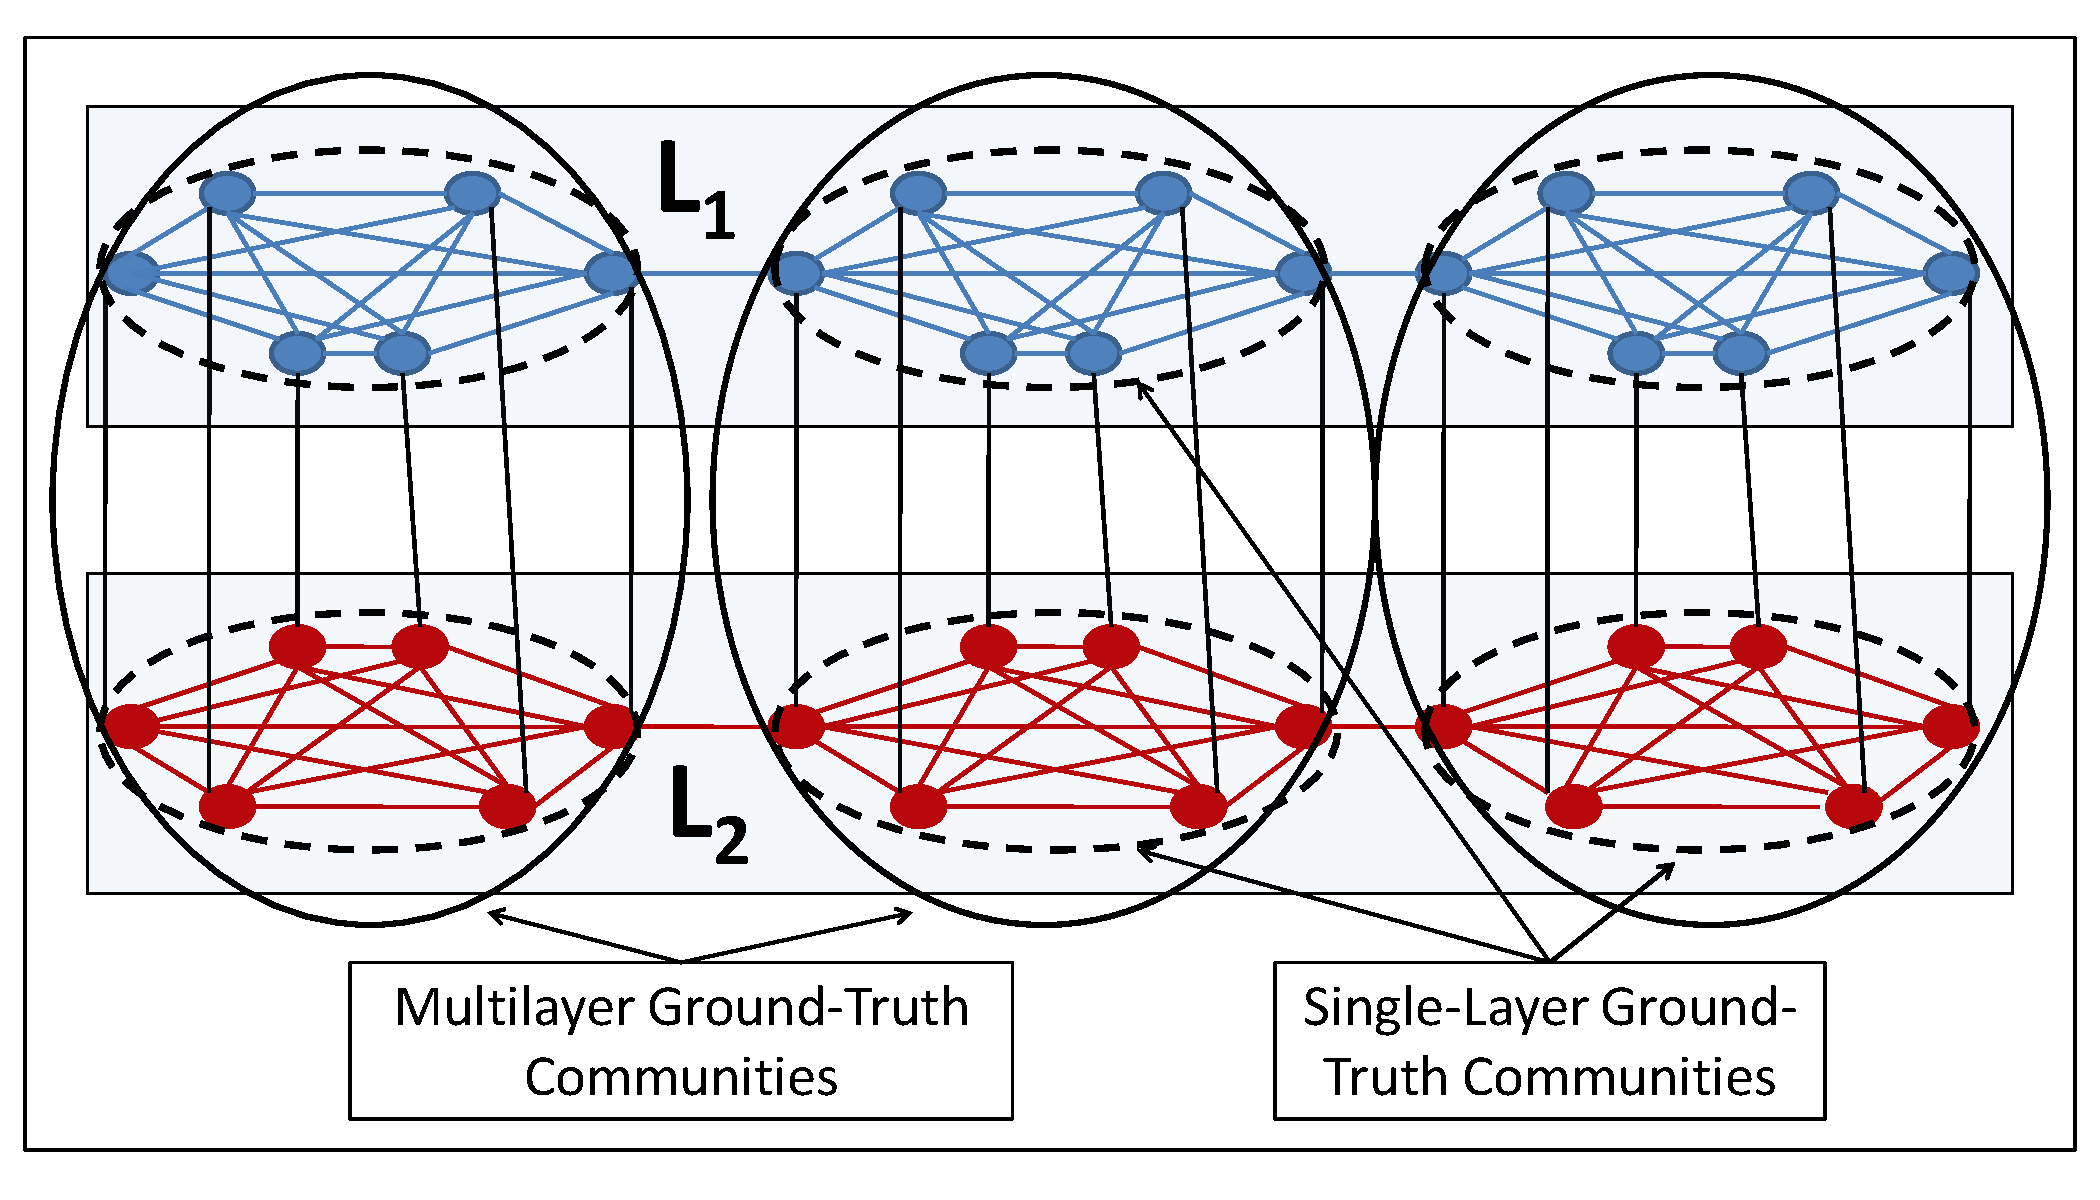
\includegraphics[width=2.3in]{./images/image31.pdf}
\vspace{-0.1in}
\caption{Network configurations with two different types of ground truth communities.}
\vspace{-0.23in}
\label{N0}
\end{figure}

\begin{figure*}
\begin{center}
% \subfigure[Avg source group-organizing group similarity of new members for successful \& unsuccessful groups
% ]{\label{T1}\includegraphics[angle=0,scale=.25]{./images2/fig3a.pdf}}
%\vspace{-0.12in}
\subfigure{\label{eval_01}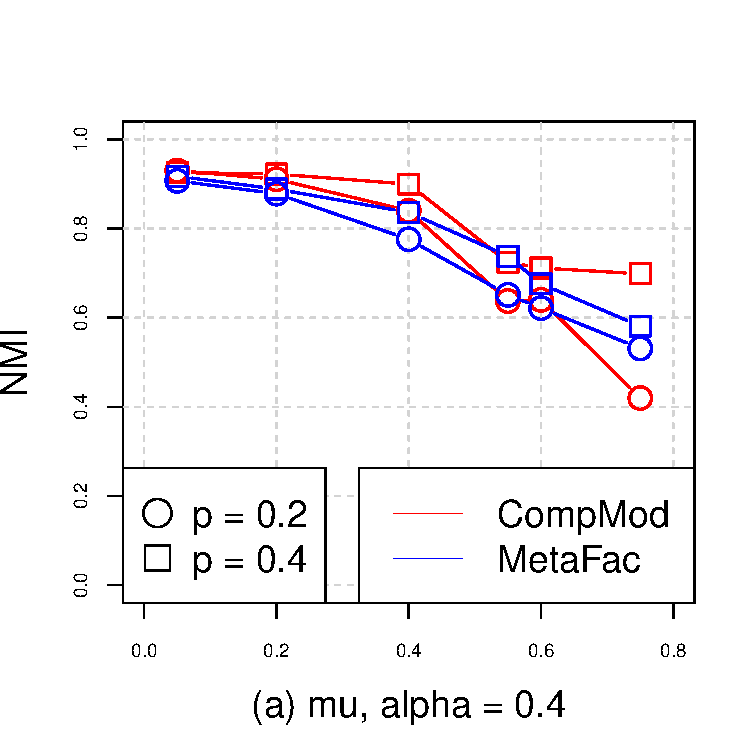
\includegraphics[angle=0,scale=.32]{./images/01.pdf}}
%\vspace{-0.12in}
\subfigure{\label{eval_02}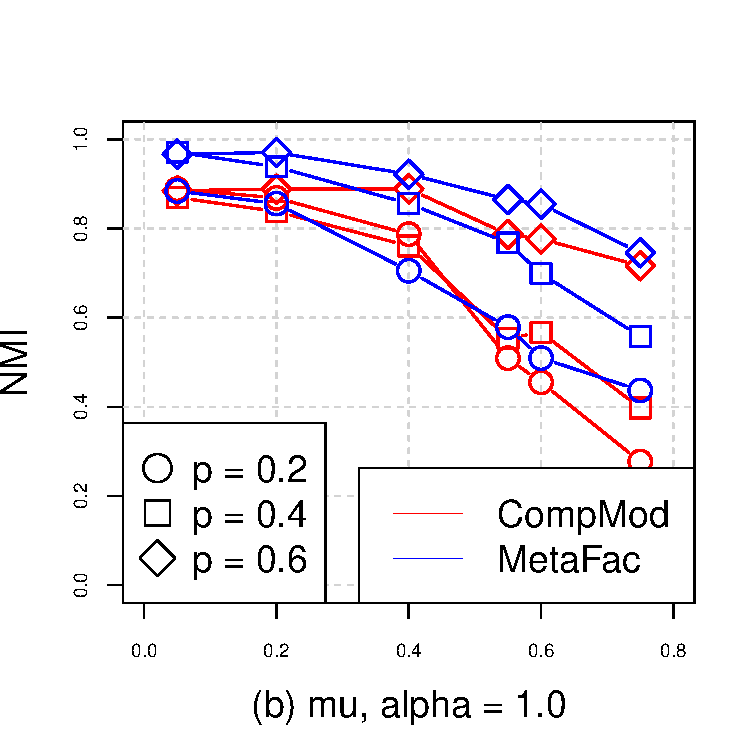
\includegraphics[angle=0,scale=.32]{./images/02.pdf}}
%\vspace{-0.12in}
 \subfigure{\label{eval_03}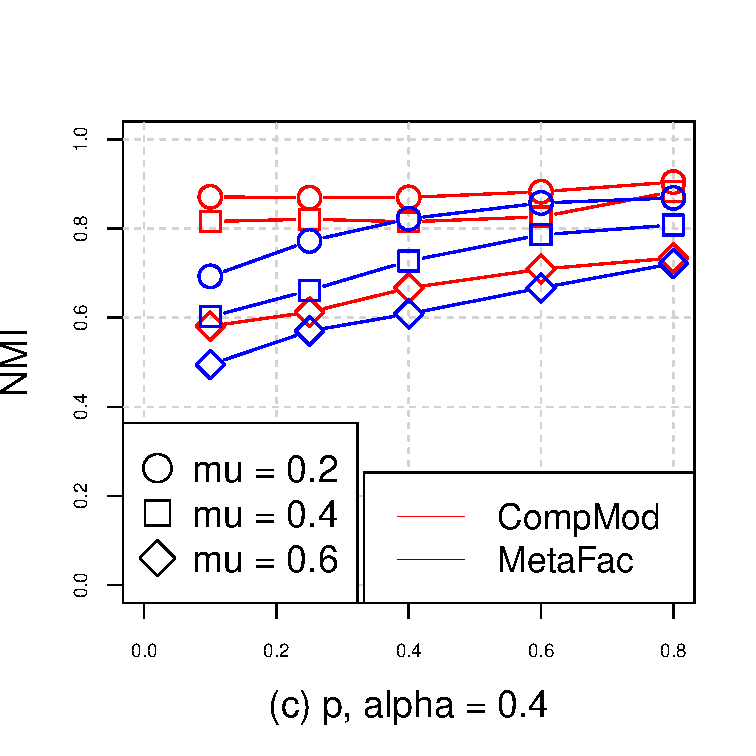
\includegraphics[angle=0,scale=.32]{./images/03.pdf}}
%\vspace{-0.12in}
\subfigure{\label{eval_04}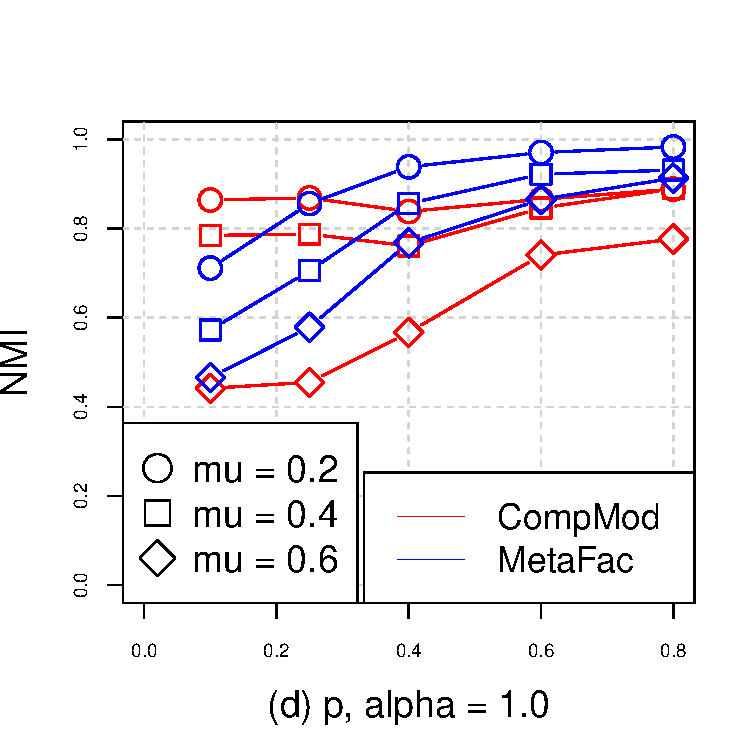
\includegraphics[angle=0,scale=.32]{./images/04.pdf}}

\end{center}\vspace{-0.22in}
\caption{Change of NMI values with $\mu$ and $p$ for `CompMod' and `MetaFac' on 2-layer networks with $100$ nodes in each layer,
generated with maximum degree $k^{i}_{max}=10$, average degree $\langle k_i\rangle=6$ \& coupling link density $d = 0.07$. }
\vspace{-0.22in}
\label{eval_syn}
\end{figure*}

% The idea is to decompose a
% multi-partite multi-relational network into multiple single-relational subnetworks, each composed of one type of edge
% and the incident nodes. Then, a composite modularity which is an integration
% of the modularity in each subnetwork is proposed for evaluating community
% structure in the multi-partite multi-relational network.
%Also, it cannot handle communities of many-to-many correspondence.

In this paper, we propose a community detection algorithm for multilayer networks
%as well as evaluate those communities with ground truth.
which is able to detect communities comprising both single type as well as multiple types of nodes,
depending on the network structure. First we represent the multilayer network with proper notations and define
the problem of community detection (sec.~\ref{dataset}). Next, we develop a methodology to construct synthetic multilayer network
with ground truth communities and evaluate it rigorously (sec.~\ref{syn_gen_eval}). The major contribution of this paper is to propose a
modularity index $Q_M$ for characterizing communities in multilayer networks. Subsequently, we develop the multilayer community detection
algorithms \textbf{GN-$Q_M$} and \textbf{Louvain-$Q_M$} incorporating the modularity index $Q_M$. We present the convergence proof for both 
the proposed algorithms along with their complexity analysis (sec.~\ref{metric}).
%[BM: one good line on we prove the convergence of \textbf{Louvain-$Q_M$} while fitting $Q_M$ into Louvain. May ask JL.]
We first evaluate the performance of the proposed modularity as a community scoring metric (sec.~\ref{ev_metric}) and then tested
the performance of the developed algorithms
against the competing algorithms.
Controlled experiments, performed on
the synthetic network, exhibit the ability of the \textbf{GN-$Q_M$} and \textbf{Louvain-$Q_M$} algorithms to
efficiently detect communities comprising both single types and multiple types on nodes (sec.~\ref{eval}). Finally,
we evaluate the proposed multilayer algorithms on the empirical dataset (Yelp and Meetup) and 
demonstrate that they outperform the state of the art baselines in correctly discovering the communities (sec.~\ref{emp}).
%[BM: one line on Meetup]
%[BM: add section numbers]
% \begin{enumerate}
%  \item Background
%  \item Existing approaches and limitations:\\
%  Most algorithms are for single layer and multiplex. Not suitable for generic multilayer. Very few works on multilayer networks
%  where nodes are different in different layers. These algorithms have the following limitations
%  \begin{enumerate}
%   \item No. of communities has to be told apriori for most of them.
%   \item Most of them either detect all single layer communities or all multilayer communities. Cannot balance optimally.
%   \item Some algorithms work only for a specific topology of multilayer networks - say, star type of networks etc.
%  \end{enumerate}
%
%  \item Scope: Proposing generic modularity and optimization technique; Proposing Benchmark synthetic multilayer networks for evaluation.
%  \item Contributions
% \end{enumerate}
%[BM: real network, recommendation?]

%The rest of the paper is organized as follows - in Sec.~\ref{dataset}, we describe the empirical and synthetic networks we use for
%evaluating our algorithm. Sec.~\ref{experiment} experimentally establishes the need of developing a new modularity
%index for multilayer networks. Sec.~\ref{metric} describes our proposed metric and community detection algorithm. In Sec.~\ref{eval},
%we evaluate our approach with respect to existing techniques and finally, in Sec.~\ref{conclus}, we conclude this paper along with
%future directions.

% %
% % There are studies on community detection in homogeneous multi-relational networks or multiplex networks (sometimes called
% % multi-dimensional networks~\cite{tang2012community}, or multi-slice networks~\cite{mucha2010community}). For example, researchers
% % developed methods for detecting communities in
% % a particular subclass of such networks, known as signed networks where each edge has a positive or negative
% % sign~\cite{traag2009community, yang2007community, bogdanov2010towards}.
% % Mucha et al. proposed a multiplex model for describing a homogeneous multi-relational network and developed a method based
% % on optimizing a generalized modularity known as stability~\cite{mucha2010community}.
% % In \cite{boden2012mining}, Boden et al. considers graphs with multiple edge types and edge attributes. In such graphs, densely
% % connected clusters are detected that also have similar attribute values.
% % Moreover, researchers proposed methods based on matrix
% % approximation~\cite{tang2012identifying}, seed-centric approach~\cite{hmimida2015community} and spectral analysis~\cite{tang2012community}.
